% !TEX encoding = UTF-8
% !TEX TS-program = pdflatex
% !TEX root = ../tesi.tex

%**************************************************************
\chapter{Tecnologie e strumenti}
\label{cap:tecnologie_e_strumenti}
%**************************************************************
In questo capitolo verranno illustrate le tecnologie e gli strumenti che sono stati utilizzati per realizzare il progetto di stage.\\
Il capitolo si apre con una descrizione di che cos'è una \textit{Blockchain} e del perché è stata scelta come tecnologia chiave per la realizzazione del progetto e, di seguito, verranno descritti tutti gli strumenti utilizzati.\\\\
Questa sezione è frutto di studi di vari documenti e \textit{whitepaper} forniti dall'azienda \cite{spidchain_whitepaper, SSID, jolocom_whitepaper, ITF_gartner, hashgraph_whitepaper}
%**************************************************************
\section{Cos'è una Blockchain}
Una \textit{Blockchain} è un \emph{\gls{dlt}}\glsfirstoccur che si basa fortemente sul \textit{consenso} e su un sistema di \textit{smart contracts}\cite{linuxFoundation}.
È quindi una piattaforma costruita su una rete di nodi (detti blocchi) distribuiti e gli elementi chiave che la contraddistinguono sono:
\begin{itemize}
	\item \textbf{Smart Contracts} - programmi che vengono eseguiti solamente quando si verificano determinate condizioni;
	\item \textbf{Consenso} - sistema che assicura che la maggioranza (50\% + 1) dei nodi della rete identifichi e sia in accordo con tutti gli altri nodi della rete che un determinato stato del sistema sia quello esatto.
\end{itemize}
Questi blocchi sono formati da quattro sezioni:
\begin{itemize}
	\item \textbf{Block size} che rappresenta la grandezza in bytes del blocco;
	\item \textbf{Block Header} è un campo particolare che è a sua volta formato da:
	\begin{itemize}
		\item \textbf{Version} numero di versione del software utilizzato;
		\item \textbf{Previous Block Hash} contiene l'hash dell'header del blocco precedente;
		\item \textbf{Markle root} hash della radice del \textit{Markle tree} (spiegato di seguito);
		\item \textbf{Timestamp} tempo di creazione del blocco;
		\item \textbf{Difficulty target} numero che indica il livello di difficoltà per l'aggiunta del blocco alla \textit{Blockchain};
		\item numero casuale o pseudo-casuale dato come risultato dell'elaborazione della \emph{\gls{pow}}\glsfirstoccur.
	\end{itemize}
	\item \textbf{Transaction counter} contiene il numero di transazioni che compongono il blocco;
	\item \textbf{Transaction} lista di tutte le transazioni che verranno processate nel blocco.
\end{itemize}
\subsection{Caratteristiche chiave}
Abbiamo spiegato che cos'è una \textit{Blockchain} ma perché questa dovrebbe essere una buona candidata per la realizzazione del modulo \gls{ITF}?\\
La risposta sta in tre caratteristiche che sono parte integrante del concetto stesso di \textit{Blockchain} e che la rendono un'ottima struttura anti-manomissione:
\begin{itemize}
	\item Funzione crittografica di hash;
	\item Strutture dati con hash pointer;
	\item Protocollo di consenso distribuito.
\end{itemize}
Le funzioni \textit{crittografiche di hash}, unite agli \textit{hash pointer} fanno sì che la struttura dati complessiva sia immutabile il che è la base dell'anti-manomissione della \textit{Blockchain}.
Se un utente malevolo modifica un dato in uno qualsiasi dei blocchi della \textit{Blockchain} questo farà sì che il puntatore hash del blocco successivo sia errato. Questo permette sia di individuare un tentativo di manomissione delle informazioni sia di capire quale blocco è stato manomesso.\\
Per comprendere meglio questi concetti, vediamo nel dettaglio le tre caratteristiche.
\subsubsection{Funzione crittografica di hash}
È una funzione matematica che converte un input di qualsiasi grandezza in un output di grandezza fissa.\\
Le funzioni crittografiche di hash hanno due proprietà fondamentali:
\begin{itemize}
	\item \textbf{Collision-resistant} - è difficile, quasi impossibile, che due input diversi creino lo stesso output;
	\item \textbf{Enable hiding} - non è possibile, partendo dall'output, recuperare l'input iniziale.
\end{itemize}
Un esempio di algoritmo che rispetta queste caratteristiche è \emph{\gls{sha256}}\glsfirstoccur.

\subsubsection{Strutture dati con hash pointer}
Gli \textit{Hash pointer} sono particolari strutture dati che contengono:
\begin{itemize}
	\item un puntatore a dove sono immagazzinati i dati;
	\item l'\textit{hash} crittografico dei dati alla quale il puntatore fa riferimento
\end{itemize}
Questo fa sì che sia possibile, oltre che recuperare le informazioni, verificare, tramite l'\textit{hash}, che le informazioni recuperate siano corrette e non manomesse.\\
Grazie a questa tipologia di struttura dati, la \textit{Blockchain} realizza un'altra struttura di fondamentale importanza per il funzionamento del sistema: il \textit{Markle Tree}.\\
Questa tipologia di struttura non è altro che un albero binario che, tramite l'ausilio degli \textit{hash pointer}, mantiene al suo interno i dati e le transazioni di ogni blocco che fa parte della \textit{Blockchain} (vedi Figura \ref{img:markeTree}).\\
I dati, contenuti nelle foglie dell'albero, vengono crittografati tramite \textit{hash} e posti su un nodo padre di livello superiore. Qui i nodi padre vengono raggruppati a coppie viene calcolato il loro \textit{hash} e vengono posti a loro volta in un livello superiore. 
Continuando a raggruppare i nodi padre e facendo l'\textit{hash} si arriva fino alla radice dell'albero che va a formare il \textit{Markle tree root.}
Se qualcuno prova a manomettere uno qualsiasi dei blocchi di dati sottostanti farà sì che l'\textit{hash pointer} ai livelli più alti non corrisponda più a quello calcolato.
\begin{figure}[!h]
	\centering
	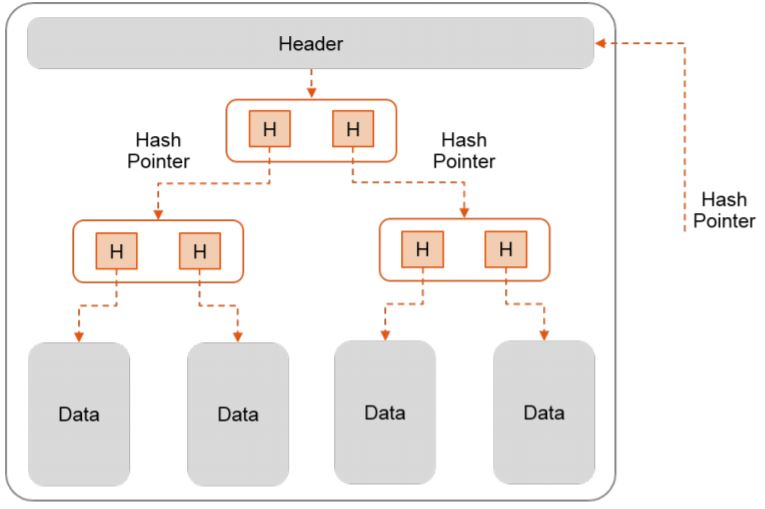
\includegraphics[scale=0.50]{immagini/markle_tree}
	\caption{Rappresentazione di un Markle Tree}
	\label{img:markeTree}
\end{figure} 
\subsubsection{Protocollo di consenso distribuito}
Uno dei punti di forza della \textit{Blockchain} è la decentralizzazione del sistema che crea. Per questo motivo è di fondamentale importanza avere un \textit{protocollo di consenso distribuito} che fa sì che ogni nodo partecipante nella rete sia d'accordo su cosa deve essere scritto nella \textit{Blockchain}.
L'algoritmo di consenso assicura due proprietà, sotto la condizione che tutti i nodi abbiamo ricevuto qualche forma di informazione:
\begin{enumerate}
	\item L'algoritmo termina quando tutti i nodi "onesti" (non malevoli e quindi nodi che non vogliono introdurre informazioni errate all'interno della rete) concordano (accettare l'informazione e scriverla sulla Blockchain o rifiutarla) sull'informazione ricevuta;
	\item L'algoritmo assicura che l'informazione sia generata da un nodo "onesto".
\end{enumerate}
In questo caso, un nodo "onesto" viene scelto per "agganciare" il nuovo blocco, contenente i nuovi dati ricevuti, alla \textit{Blockchain} e gli altri nodi replicano il cambiamento di stato sulla propria rete \textit{Blockchain}. In questo modo si riesce a generare fiducia tra tutti i nodi quando, tra di loro, non si conoscono e non si fidano.

\subsection{Tipologie di Blockchain}
La rete \textit{Blockchain} è disponibile in due versioni differenti:
\begin{itemize}
	\item \textbf{Permissionless Blockchain} - è detta anche \textit{Blockchain pubblica} perché tutti possono partecipare alla rete. Non vi è alcun tipo di controllo che governa la partecipazione alla rete o che ne limiti l'accesso.  Il comportamento dell'interno sistema è tutto in mano al protocollo di consenso distribuito;
	\item \textbf{Permissioned Blockchain} - è detta anche \textit{Blockchain privata} perché per poter avere accesso alla rete e potervi quindi partecipare è necessaria la verifica da parte di nodi già interni alla rete che autorizzino o meno l'accesso a nuovi nodi.
\end{itemize}
La scelta tra \textit{permissioned} o \textit{permissionless} è guidata principalmente dal tipo di applicazione o servizio che si vuole sviluppare o fornire e dalla necessità o meno di avere controllo su chi può partecipare alla rete.
Per l'implementazione di un \gls{ITF} sono necessarie sei caratteristiche. 
Sia le \textit{permissioned Blockchain} che quelle \textit{permissionless} implementano queste caratteristiche ma con leggere differenze che possono determinare la scelta verso una o l'altra tecnologia.

\subsection{Permissionless vs Permissioned}
In Figura \ref{img:permisionedVSpermissionless} viene riportata un'immagine che racchiude le sei caratteristiche necessarie per poter creare un \gls{ITF} sicuro ed efficiente insieme ad una valutazione, data da \emph{\gls{gartner}}\glsfirstoccur, che mostra come le varie tipologie di \textit{Blockchain} implementano tale caratteristica.
\begin{figure}[h]
	\centering
	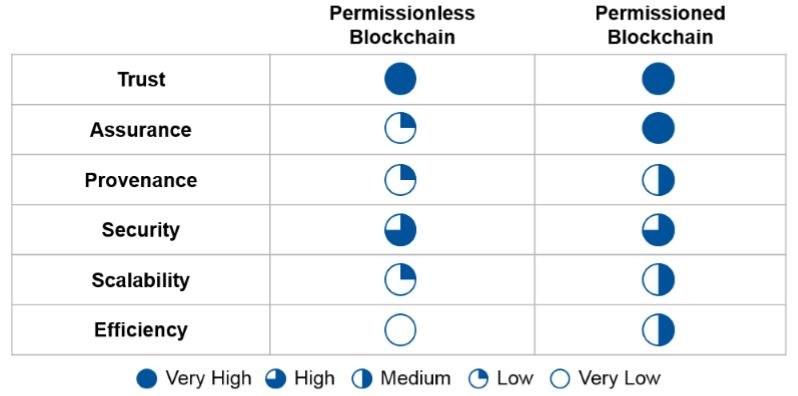
\includegraphics[scale=0.50]{immagini/blockchain_ability_to_implement_ITF}
	\caption{Schema comparativo Permissionless vs Permissioned}
	\label{img:permisionedVSpermissionless}
\end{figure} 
\\
Come si può vedere dallo schema la tecnologia migliore da adottare per implementare l'\gls{ITF} è una \textit{permissioned Blockchain}.
I motivi che portano a questa scelta sono:
\begin{itemize}
	\item \textbf{Fiducia (Trust)} - la \textit{permissioned Blockchain} risulta più appropriata per gestire la fiducia ed il rischio in un \gls{ITF} a causa del suo modello di governance che pone un certo controllo su chi può e chi non può accedere alla rete; 
	\item \textbf{Sicurezza (Assurance)} - una \textit{permissionless Blockchain} assicura un livello inferiore di assurance proprio perché permette a qualsiasi nodo, anche uno potenzialmente maligno, di partecipare alla rete cosa che, una \textit{permissioned Blockchain}, non permette;
	\item \textbf{Provenienza (Provenance)} - le \textit{permissionless Blockchain} non condividono un servizio centrale di timing. Le \textit{permissioned Blockchain} riescono, tramite un accordo, ad utilizzare un clock centrale che sincronizza i loro timestamp;
	\item \textbf{Scalabilità (Scalability)} - una \textit{permissioned Blockchain} risulta più efficace se sottoposta ad un grande carico di lavoro grazie ai suoi algoritmi di consenso più snelli che non devono garantire la fiducia tra i singoli nodi ma solo che il blocco da inserire, nella \textit{Blockchain}, sia corretto;
	\item \textbf{Efficienza (Efficency)} - conseguenza diretta della Scalabilità e quindi della leggerezza degli algoritmi di consenso, una \textit{permissioned Blockchain} risulta più efficiente, per quanto riguarda i consumi energetici, rispetto alla sua controparte \textit{permissionless}.
\end{itemize}
\subsection{Scelta tecnologica}
Dal punto di vista prettamente tecnologico la tipologia migliore di \textit{Blockchain} che sarebbe da utilizzare per implementare il modulo \gls{ITF} è quella di tipo \textit{permissioned}.\\
Questa scelta deriva dalle numerose considerazioni, studi e analisi che sono stati condotti durante buona parte del primo mese di stage.\\
Durante questo periodo di tempo sono state studiate molte tecnologie sia di tipo \textit{permissioned} che di tipo \textit{permissionless} tra le quali menziono:
\begin{itemize}
	\item \textbf{Hyperledger Fabric} - è un framework di proprietà della Linux Foundation \cite{linuxFoundation} e fa parte del \emph{\gls{hyperledgerProject}}\glsfirstoccur per la creazione di \textit{Blockchain} di tipo \textit{permissioned}. Fornisce un'architettura modulare che permette alle varie entità di condurre transazioni confidenziali senza passare le informazioni attraverso un'autorità centrale. Questo può essere ottenuto grazie alla creazione di canali confidenziali nella quale possono partecipare soltanto le parti coinvolte in una transazione;
	\item \textbf{Ethereum} - Fondata da Vitalk Buterin, \textit{Ethereum} è una delle piattaforme \textit{Blockchain permissionless} più mature disponibili oggi.
	È conosciuta soprattutto per la sua robustezza e flessibilità nella creazione degli \textit{smart contracts} e per questo è utilizzata per modellare molti use-case aziendali \cite{ethereumProject}.
\end{itemize}
Nonostante tutti gli studi, i confronti e le analisi effettuate sulle varie tecnologie, conducessero a scegliere una \textit{Blockchain} di tipo \textit{permissioned} e, più nel dettaglio, \textit{permissioned} creata tramite \textit{Hyperledger Fabric}, la scelta tecnologia finale è ricaduta sulla tecnologia di tipo \textit{permissionless} creata tramite la piattaforma \textit{Ethereum}.\\
Questa scelta è stata presa dopo numerosi dibatti e riunioni interne all'azienda in cui, sia io che l'altro stagista che ha partecipato alla realizzazione del progetto, ci siamo interrogati sulla fattibilità del progetto con una tecnologia di tipo \textit{permissioned} realizzata tramite \textit{Hyperledger Fabric}.\\
Le motivazioni che ci hanno spinto a scegliere \textit{Ethereum} come tecnologia finale, nonostante le analisi condotte precedentemente, sono state:
\begin{itemize}
	\item \textit{Ethereum} è una tecnologia molto più matura, solida e conosciuta rispetto ad \textit{Hyperledger Fabric};
	\item possiede una community di sviluppatori di tutto rispetto, molto più grande e attiva rispetto ad \textit{Hyperledger Fabric};
	\item realizzare il progetto in \textit{Ethereum} sarebbe stato molto più semplice e veloce rispetto a realizzarlo in \textit{Hyperledger Fabric}. Questo deriva dal fatto che, essendo \textit{Ethereum} una piattaforma \textit{permissionless}, possiede già una propria \textit{Blockchain} che può essere utilizzata da chiunque.\\
	\textit{Hyperledger Fabric}, essendo \textit{permissioned}, avrebbe richiesto la creazione di una rete \textit{Blockchain} ad hoc oltre che la creazione di tutta la logica del modulo \gls{ITF} che era il core dello stage;
	\item si è fatto un confronto tra costi (in denaro) delle due tecnologie.\\
	\textit{Ethereum} fa pagare ogni transazione che viene eseguita nella sua \textit{Blockchain permissionless} come tassa di utilizzo.\\
	\textit{Hyperledger Fabric} non richiede alcun tipo di pagamento per eseguire codice o transazioni nella rete in quanto, essendo \textit{permissioned}, si sarebbe dovuto creare una rete privata di nostra proprietà per realizzare il progetto. Il costo quindi si sposta nel mantenimento dell'intera rete e non più sul suo utilizzo.
\end{itemize}
Oltre a queste motivazioni, un' altra ci ha spinto a scegliere la tecnologia \textit{Ethereum} ovvero la volontà che avevamo di lasciare qualcosa di concreto in mano all'azienda una volta finito il periodo di stage, qualcosa che funzionasse e che non fosse solo un "abbiamo provato". La tecnologia \textit{Ethereum} essendo di più facile comprensione e utilizzo ci avrebbe permesso di concentrarci di più sull'effettiva implementazione della logica e dei test e così è stato tanto che alla fine del periodo di stage siamo riusciti a realizzare e consegnare una \gls{poc} funzionante e, per quanto siamo riusciti a verificare, solida.

\section{Strumenti e tecnologie utilizzate}
Passiamo ora a descrivere tutte le tecnologie e gli strumenti che sono stati utilizzati per la modellazione concettuale, l'implementazione, il testing ed il deployement del modulo \gls{ITF} realizzato utilizzando la piattaforma \textit{Ethereum}.

\subsection{Strumenti per la gestione ed il versioning}
\subsubsection{Node.js}
Node.js (logo in Figura \ref{img:nodejs}) è un runtime Javascript costruito sul JavaScript Engine \cite{nodeGuida}, che è il runtime di Google utilizzato anche da Chrome e disponibile sulle varie piattaforme.
\begin{figure}[h]
	\centering
	
\includegraphics[scale=0.05]{immagini/nodejs}
	\caption{Logo di Node.js}
	\label{img:nodejs}
\end{figure}
\\
La caratteristica principale di Node.js risiede nella possibilità che offre di accedere alle risorse del sistema operativo in modalità \emph{\gls{event-driven}}\glsfirstoccur\cite{nodeEvent} e non sfruttando il modello basato su processi o \textit{thread} concorrenti, utilizzato dai classici Web Server. L'ecosistema dei pacchetti di Node.js, \textbf{npm}, è il più grande ecosistema di librerie \gls{event-driven} al mondo.
\subsubsection{Git}
\gls{git} è un software di controllo di versione distribuito, creato nel 2005 da Linus Torvalds \cite{gitSite}. Viene utilizzato da Athesys S.r.l per il controllo di versione dei progetti (vedi Figura \ref{img:git}).
\begin{figure}[h]
	\centering
	
\includegraphics[scale=0.05]{immagini/git}
	\caption{Logo Git}
	\label{img:git}
\end{figure}

È usabile principalmente da interfaccia a linea di comando, ed oggi è in assoluto uno dei software per il controllo di versione più utilizzati.\\
Come tutti i software per il controllo di versione, si basa sul concetto di \emph{\gls{repository}}\glsfirstoccur\cite{gitSite}, ovvero un ambiente in cui vengono immagazzinati i \emph{\gls{metadati}}\glsfirstoccur\cite{gitGuida} che possono essere recuperati e aggiornati da chi può averne accesso.
\begin{enumerate}
	\item \textbf{Committed} - significa che il file è al sicuro nel database locale;
	\item \textbf{Modified} - significa che il file è stato modificato, ma non è ancora stato "committato" nel database quindi non è ancora salvato;
	\item \textbf{Staged} - significa che il file è stato contrassegnato in modo tale che venga inserito come istantanea alla prossima \emph{\gls{commit}}\glsfirstoccur
\end{enumerate}
Quanto detto porta alle quattro sezioni principali di un progetto \gls{git}: la \textit{working directory}, la \textit{staging area}, la \textit{local repo} e la \textit{remote repo}.

\subsection{Strumenti per la modellazione concettuale}
\subsubsection{Astah Professional}
Per la progettazione è stato necessario modellare i casi d'uso tramite \emph{\gls{uml}}\glsfirstoccur e la scelta del software da utilizzare è ricaduta su Astah Professional (vedi Figura \ref{img:astah}), disponibile in versione gratuita grazie alla licenza accademica.
\begin{figure}[h]
	\centering
	
\includegraphics[scale=1]{immagini/astah}
	\caption{Logo Astah Professional}
	\label{img:astah}
\end{figure}
\\
Astah Professional supporta sia i costrutti di \gls{uml} 1 che di \gls{uml} 2 e permette di modellare casi d’uso, i diagrammi delle classi, degli oggetti, delle attività e di sequenza; inoltre, produce diagrammi che risultano adatti ad essere inseriti in relazioni formali.
\subsection{Ambiente di lavoro}
\subsubsection{Sistema Operativo}
Durante tutta la durata dello stage si è fatto uso del sistema operativo \textbf{Windows 10} per pura preferenza personale in quanto, se ve ne fosse stata la necessità o la preferenza, sarebbe stato possibile lavorare in ambiente Linux.
\subsubsection{IDE}
Per quanto riguarda l'ambiente di sviluppo, la norma aziendale prevede che ogni persona venga lasciata libera di adottare ciò che ritiene più adatto nello svolgimento del proprio lavoro.\\
La mia scelta è ricaduta sull'editor \textit{Visual Studio Code} (si può vedere la sua classica interfaccia in Figura \ref{img:visualstudiocode}) poiché è un software \gls{opensource} costantemente aggiornato e stabile. Inoltre il grande numero di estensioni disponibili è un punto di forza dell'editor, in quanto permettono di aggiungere funzionalità che lo rendono uno strumento comodo e veloce da utilizzare.
\begin{figure}[h]
	\centering
	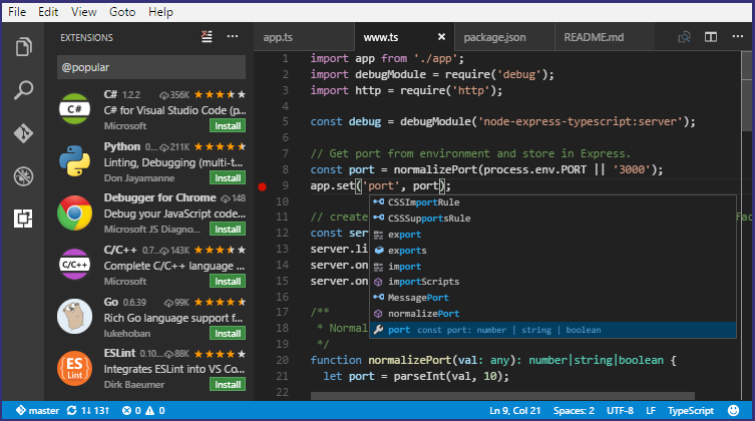
\includegraphics[scale=0.5]{immagini/vsc_interface}
	\caption{Interfaccia Visual Studio Code}
	\label{img:visualstudiocode}
\end{figure}
\\
Oltre a questo, \textit{Visual Studio Code}, ha un integrazione diretta con \gls{git}. Questo fa sì che ci sia una finestra dedicata per il controllo delle differenze tra i file modificate che permette di fare il \textit{commit} delle modifiche online sia su server \gls{git} privati che su \gls{repository} presenti su GitHub \cite{gitGuida, gitSite}.
\subsection{Framework di sviluppo e testing}
\subsubsection{Truffle Suite}
Truffle (logo in Figura \ref{img:truffle}) è un \emph{\gls{framework}}\glsfirstoccur  di test \textit{Ethereum} nato allo scopo di supportare lo sviluppo di \emph{\gls{dapp}}\glsfirstoccur  Ethereum molto supportato ed utilizzato dalla community.
Può essere utilizzato per creare, testare e rilasciare \gls{dapp} all'interno della rete \textit{Ethereum} o nelle reti di testing \cite{truffle}.
Le sue principali caratteristiche sono:
\begin{itemize}
	\item Testing automatico degli \textit{smart contracts};
	\item Possiede una pipeline configurabile per fare building di applicazioni web e console;
	\item Possiede dei generatori per la creazione di account di testing fittizi;
	\item Possiede una console in grado di interagire con i contratti già compilati;
	\item Permette l'esecuzione di script JavaScript utilizzati principalmente per il testing;
\end{itemize}
La caratteristica più importante è il fatto che permette di creare ambienti di test in modo molto rapido e semplice il che è una caratteristica fondamentale quando si vuole progettare una \gls{dapp} in quanto, una volta rilasciata nella rete \textit{Blockchain}, non è più possibile modificare o aggiornare quanto fatto se non rilasciando una nuova \gls{dapp} che va a "sostituire" quella mal funzionante \cite{truffle}.
\begin{figure}[h]
	\centering
	
\includegraphics[scale=0.3]{immagini/truffle}
	\caption{Logo Truffle suite}
	\label{img:truffle}
\end{figure}
\subsubsection{Ganache}
È una \textit{Blockchain Ethereum} installata direttamente in locale utilizzata per la fase di test e debug delle \gls{dapp} prima di rilasciarle nella rete \textit{Ethereum principale}(vedi Figura \ref{img:ganache}).
Le caratteristiche di questo tool sono \cite{ganache}:
\begin{itemize}
	\item Permette la creazione di una versione personale della \textit{Blockchain Ethereum} con tutte le sue caratteristiche e configurazioni;
	\item Ha un'interfaccia grafica che permette di visualizzaretutti gli account, indirizzi, chiavi private, transazioni e bilanci della rete e di monitorare l'evoluzione della rete man mano che avvengono transazioni;
	\item Dà la possibilità di visualizzare, tramite log, lo stato interno della \textit{Blockchain} e tutte le informazioni utili per il debugging;
	\item Dà la possibilità di configurare tutte le impostazioni del \emph{\gls{mining}}\glsfirstoccur dei blocchi a seconda delle esigenze;
	\item Viene distribuito con un \textit{Block Explorer} che permette di esaminare tutti i blocchi e le transazioni in modo da avere una visione interna di quello che succede nella rete.
\end{itemize}
Questo strumento è stato molto utile per le fasi di testing e di debugging del modulo \gls{ITF} in quanto, essendo una delle prime \gls{dapp} che stavo per realizzare, avere chiaro come funzionasse una \textit{Blockchain} e come venissero modificate le informazioni al suo interno era di fondamentale importanza. Questo strumento ha permesso, in modo molto semplice grazie alla sua interfaccia grafica, di ottenere tutte le informazioni necessarie.
\begin{figure}[h]
	\centering
	
\includegraphics[scale=0.5]{immagini/ganache}
	\caption{Logo Ganache}
	\label{img:ganache}
\end{figure}
\subsection{Linguaggi di programmazione}
\subsubsection{Solidity}
È un linguaggio di programmazione ad alto livello \emph{\gls{contract_oriented}}\glsfirstoccur  utilizzato per implementare gli \textit{smart contracts} nelle reti \textit{Blockchain} basate su \textit{Ethereum} (vedi Figura \ref{img:solidity}).
Questo linguaggio è "statically typed", supporta l'ereditarietà, l'implementazione di librerie, la creazione di tipi definiti dall'utente ed è stato creato per interagire direttamente con l'\emph{\gls{evm}}\glsfirstoccur. 
Ha una sintassi simile a \textit{JavaScript} con forti richiami a \textit{C++} e \textit{Python}\cite{solidity}.
Le sue caratteristiche principali sono \cite{solidity}:
\begin{itemize}
	\item è un linguaggio di programmazione ad alto livello, molto intuitivo e "user-friendly";
	\item è un linguaggio ad oggetti che permette la modellazione di realtà complesse con minimo sforzo;
	\item è molto semplice da imparare ed utilizzare in quanto è basato su \textit{JavaScript};
	\item essendo un linguaggio "statically typed" il processo di verifica delle variabili avviene a \textit{compile-time} e non a \textit{run-time};
	\item è possibile integrare Solidity in ambienti di sviluppo come IntelliJ IDEA, Microsoft Visual Studio e Microsfot Visual Studio Code;
	\item permette di interagire con \gls{evm}.
\end{itemize}
\begin{figure}[h]
	\centering
	
\includegraphics[scale=0.25]{immagini/solidity}
	\caption{Logo Solidity}
	\label{img:solidity}
\end{figure}
Questo linguaggio di programmazione è stato l'unico utilizzato per tutto il periodo di stage in quanto il lavoro che mi era stato affidato era quello di creare tutta la logica dell'\gls{ITF} e dell'interazione tra "mondo esterno" e \textit{Blockchain}.\\
Il linguaggio è stato utilizzato anche per la codifica dei relativi test.\\
La versione utilizzata era l'ultima disponibile ovvero la versione \textit{0.4.24}.
